\documentclass{ppig}
\usepackage{epsfig, graphicx} % support for image encoding and manipulation
\usepackage{ucs} % support for using UTF-8 as input encoding in LaTeX
\usepackage[utf8x]{inputenc} % required for UTF-8 support with ucs.sty
\usepackage{tabularx, multirow, booktabs} % support for high-quality tables

% The titlebox defines how much vertical space is given for
% the authors' list. If you need extra space to show all the
% authors, uncomment the line below and increase the value. Please
% do not make the titlebox smaller than the original size of 5cm.
%\setlength\titlebox{5cm}

\title{An Examination of IDE Design for Programming as Problem-Solving}

% List the authors like you would in a table.
% The \And command creates another author's column. Use it after the
% details of one author to separate them from the following author horizontally.
% The \AND command creates a new "row" of authors and it should be used
% when the authors don't fit on the same line. You may have to increase
% the titlebox so that the author's don't overlap with the abstract.
\author{Nicholas Nelson \\
  Electrical Engineering \&\\ Computer Science \\
  Oregon State University \\
  nelsonni@oregonstate.edu \\
  \And
  Anita Sarma \\
  Electrical Engineering \&\\ Computer Science \\
  Oregon State University \\
  Anita.Sarma@oregonstate.edu \\
  \And
  André van der Hoek \\
  Department of Informatics \\
  University of California, Irvine \\
  andre@ics.uci.edu
}
  
\date{\today}

% Packages and macros for editorial purposes. Not required for submission.
\usepackage{color}
\definecolor{darkgreen}{rgb}{0.0, 0.5, 0.0}
\definecolor{ballblue}{rgb}{0.13, 0.67, 0.8}
\definecolor{aoblue}{rgb}{0.0, 0.0, 1.0}
\newcommand{\bold}[1]{\textit{\textbf{\color{aoblue}#1}}} % macro for boldifications
\newcommand{\todo}[1]{\textit{\textbf{\color{red}TODO: #1}}} % macro for TODO items
\newcommand{\discuss}[1]{\textit{\textbf{\color{darkgreen}#1}}} % macro for in-line discussions/questions
\newcommand{\nameUI}{\textit{<Insert Name>} UI} % macro placeholder for the name of the UI
\usepackage{enumitem}

\begin{document}
\maketitle
\thispagestyle{empty}

\begin{abstract}

Programming is more than generating, testing, and maintaining code.
Programming is fundamentally an extension of cognitive problem-solving skills applied to computational problems.
Contemporary IDEs natively support the code-centric aspects of programming, but forego supporting many of the cognitive aspects of problem-solving that do not directly involve code.
We propose that IDEs should support the entire gamut of problem-solving activities during programming, and that this requires a re-examination and redesign of the IDE user interface.
In this paper, we describe six activities and 22 actions that exemplify problem-solving in programming.
We further explore one activity and it's actions: the actions developers take when developing strategies to address a programming task.
In particular, we look at the actions of: (1) articulating \& refining alternatives, (2) understanding \& assessing alternatives, and (3) recombining aspects of alternatives.
Based upon our observations, we propose a new user interface for IDEs which enables previously underrepresented aspects of problem-solving; specifically addressing the disparity in support for these three aspects. 
\end{abstract}

\section{Introduction}
\bold{Scenario to illustrate programming as problem-solving}\vspace*{-0.4\baselineskip}

Imagine a scenario in which Sally, a junior developer, is tasked with updating a specific feature to take advantage of a new architecture within the core API of the larger software project. In the process of accomplishing this task, she must use several different applications and a variety of file formats.

Sally begins her project by logging into the company's issue tracker and assigning the associated issue to herself.
She also downloads and opens several documents included with the feature issue; a PDF document containing sketches and notes from the design team, a list of requirements from the marketing team, and another PDF document containing an estimated timeline from the project manager assigned to this project.
Before beginning to write code, Sally decides that she needs to understand the area of code she will be modifying and drafts a plan for how to implement those modifications.
To accomplish these sub-tasks, she spends a day reading through the code using an IDE and sketching potential implementations on a piece of paper using shapes and arrows to represent different abstractions of the code.
After exhausting her initial ideas, she works through some of the more promising sketches to determine the feasibility of each alternative.

The sketches and ideas that appear to have the most strengths (and inversely, the least weaknesses) for this specific situation will require modifying certain portions of the core architecture of the software.
Since changes to the core architecture will affect the rest of the development team, and could potentially interrupt development in other areas of the project, Sally sends emails to Mark (the senior developer on her team) and the project manager.
After several rounds of emails, and one project meeting organized by the project manager, Sally has notes scribbled on several pieces of paper, a trail of emails between different stakeholders, and a verbally-communicated history of why and how the code is organized the way it is today.

Converting all of the information contained within these different artifacts into useful code requires coalescing only the best aspects into a single solution.
Sally is able to complete her task, but not without significant effort to remain organized.
Working with non-code artifacts requires Sally to add additional tools into her workspace, which increases the complexity of accomplishing her tasks.
Throughout this scenario, Sally is forced to employ a variety of tools that accomplish particular portions of her task but none allow her to focus on the entire task.

\section{Programming as Problem-Solving}

\bold{Introduction to our model of programming as problem-solving, and the mapping between problem-solving psychology and programming tasks}

Examining the disparate and dispersed nature of artifacts in Sally's situation, which exemplifies a typical situation for programmers, we see that a new way of understanding the nature of programming is needed.
We propose using problem-solving as a lens to examine programming tools, specifically IDEs, to assist in identifying which aspects of programming are not being supported and to determine how to address those gaps.

Much is known already about programming being a problem-solving activity beyond editing code in the editor provided by the IDE.
During software development, for instance, programmers are known to create all sorts of auxiliary non-code artifacts~\cite{cherubini2007whiteboard}.
As a second example, programmers are known to organize these artifacts into structures that are relevant to the particular task(s) they are currently focused upon~\cite{baltes2016empirical}.
As a final example, programmers are known to not pursue a single solution, but to generally approach a task by exploring (either mentally or externalized) multiple alternative solutions~\cite{madeyski2017experimentation}.
By applying prior work on problem-solving from a cognitive psychology perspective~\cite{mayer1992thinking}, we can classify these actions, respectively, into \textit{representing relevant information}, \textit{contextualizing information}, and \textit{generating alternatives}.
These actions can then be generalized to represent the problem-solving activities of \textit{externalizing thoughts \& ideas} and \textit{developing strategies}.

\discuss{For André: Does the following paragraph say what was stated in your previous notes in the margins?\\}
Table~\ref{matrix} summarizes the full set of problem-solving activities employed during programming sessions, based on an extensive survey of literature that we performed.
The activities broadly fall into six categories, with specific types of actions providing detail to the high-level abstractions of the activities.
Clearly not every task needs all of these problem-solving actions, and there is no linearity to the order in which they are employed.
Sometimes these actions are not observed because they happen in the programmer's head.
At the same time, all of these activities and actions have been observed to happen, they serve as important roles in knowledge base to the programming problem at hand.

\begin{table}[!htbp]
\caption{Activities and Actions of Programming as Problem-Solving}
\label{matrix}
\centering
\begin{tabular}{|c|l|}
	\hline
	\multicolumn{1}{|c|}{\textbf{Activity}} 
	& \multicolumn{1}{c|}{\textbf{Action}}\\\hline
	\multirow{5}{*}{Understanding the situation} 
	& Identifying goals \\\cline{2-2}
	& Recalling prior knowledge \\\cline{2-2}
	& Constructing models \\\cline{2-2}
	& Interpreting code artifacts \\\cline{2-2}
	& Filling knowledge gaps \\\hline
	\multirow{3}{*}{Externalizing thoughts \& ideas} 
	& Representing relevant information \\\cline{2-2}
	& Contextualizing information \\\cline{2-2}
	& Preserving contextual information \\\hline
	\multirow{4}{*}{Developing strategies} 
	& Generating alternatives \\\cline{2-2}
	& Articulating and refining alternatives \\\cline{2-2}
	& Understanding and assessing alternatives \\\cline{2-2}
	& Recombining aspects of alternatives \\\hline
	\multirow{3}{*}{Enacting change} 
	& Translating strategies to actions \\\cline{2-2}
	& Tracking progress \\\cline{2-2}
	& Evaluating and assessing change \\\hline
	\multirow{5}{*}{Collaborate} 
	& Feedback solicitation \\\cline{2-2}
	& Team work \\\cline{2-2}
	& Group think \\\cline{2-2}
	& Leveraging group knowledge \\\cline{2-2}
	& Synchronization \\\hline
	\multirow{2}{*}{Retrospect} 
	& Reflect on work \\\cline{2-2}
	& Preserve work \\\hline
\end{tabular}
\end{table}

\section{Challenges}
\bold{Discussion of challenges associated with current IDEs/problem-solving in programming}

\discuss{For André: How should we present challenges in regards to modern IDEs (and their UI)?\\}
Modern IDEs adhere to some common design principles: clarity, consistency, progressive disclosure, and strong visual hierarchies.
Clarity to allow users to understand what they are interacting with, predict what will happen when they use it, and then successfully interact with it.
Consistent in both the design of elements shown to users and the behaviors associated with those elements.
Showing only what is necessary on each screen, and allowing users to progressively expose additional features as necessary when workflows dictate that such actions could be necessary.
Strong visual clues that direct user's gaze and interactions to follow the hierarchy of visual elements presented on a screen.
Modern IDEs seek to provide advanced features only when needed and to allow users to focus on the development of code as their primary activity.
This assumption leads to workflows and uses cases that favor code-centric design, and askew activities and interactions with non-code artifacts to other applications.

Previous work on alternative UI models for IDEs have focused on expanding the interface to allow more dynamic interactions for code comprehension and orientation.
Bragdon et al. proposed a user interface comprised of lightweight, editable fragments called bubbles, which form concurrently visible working sets in an interface called Code Bubbles~\cite{bragdon2010bubbles}.
DeLine et al. explored leveraging spatial memory to keep developers oriented by providing an infinite zoomable surface for software development, called Code Canvas~\cite{deline2010canvas}.
And combining efforts, the Code Bubbles team at Brown University and the Code Canvas team at Microsoft Research jointly created Debugger Canvas which provides collections of code bubbles on a two-dimensional pan-and-zoom interface~\cite{deline2012debugger}.
The interface models developed by these teams provide both theoretical and practical experience into alternative UI designs that help to break the mold of the ``bento-box'' model of IDEs.
Henley and Fleming similarly examined the tedious nature of navigating large information spaces and sought to reduce this burden for developers through a code editor UI that consists of a patch grid and a ribbon for navigating quickly through sets of code~\cite{henley2014patchworks}.
Da Silva et al. proposed a conflict avoidance approach to developer coordination problems which combines Emerging Design and side-by-side presentation in an architecture called Lighthouse~\cite{dasilva2006lighthouse}.
The Lighthouse user interface provides time-sensitive information about parallel changes introduced to a shared codebase in a novel approach to information awareness between developers in a team environment.
We seek to take these experiments a step further and examine whether combining the paradigm of programming as problem-solving and alternative UI design can further enable developers in developing solutions to computational problems.

\section{IDEs as Problem-Solving Tools}
\bold{Present and discuss our envisioned solution\\}
To address these challenges, we have begun a long-term research effort that attempts to rethink the IDE from the ground up using the problem-solving perspective as a paradigm shift for evaluating our design rationale.
We use Code Bubbles~\cite{bragdon2010bubbles} and Code Canvas~\cite{deline2010canvas} as key inspirations for interface designs that eschew window-based interfaces and explore spatial interfaces allowing users to project meaning onto the layout of their development environment.
Extending the zoomable canvas of Code Canvas and the code bubble windows of Code Bubbles, we explore these and other concepts from interface design to support the problem-solving activities that programmers encounter.

Modern IDEs are comprised of different information sources being presented in a variety of visual elements that must be organized and comprehended by users.
According to the Gestalt school of thought, our perception of the world is influenced by the way we group and segregate the visual stimuli presented to us~\cite{kimchi2003perceptual}.
Instead of perceiving individual and distinct objects in the world, we perceive objects that are logically connected to each other~\cite{kimchi2003perceptual}.
The strength of grouping objects is inversely proportional to the distance between the elements~\cite{bergman2009peirce}; therefore, the closer the elements are to each other the stronger our perception is that these belong to the same group.
To take advantage of the neuro-cognitive process of perceptual organization, we propose a cards-based interface which allows card positioning and stacking for logical organization across user-driven tasks.

Programming activities span editing code to sketching ideas on whiteboards, with each action serving different problem-solving aspects in pursuit of a solution.
In order to support this variety of actions, we propose that cards in our cards-based interface come in different types that support specific information sources and interactions while providing a common platform.
These card types can include code editors for working with code in specific programming languages, sketchpads for both drawing ideas and annotating text, webpages for referencing information sources on the Internet, todo lists for organizing tasks, timelines for managing projects, emails and chat transcripts for communications, etc.

\begin{figure}[h!]
	\caption{Cards-based User Interface of a Problem-Solving IDE}
	\label{mockup}
	% trim={<left> <lower> <right> <upper>}
	\fbox{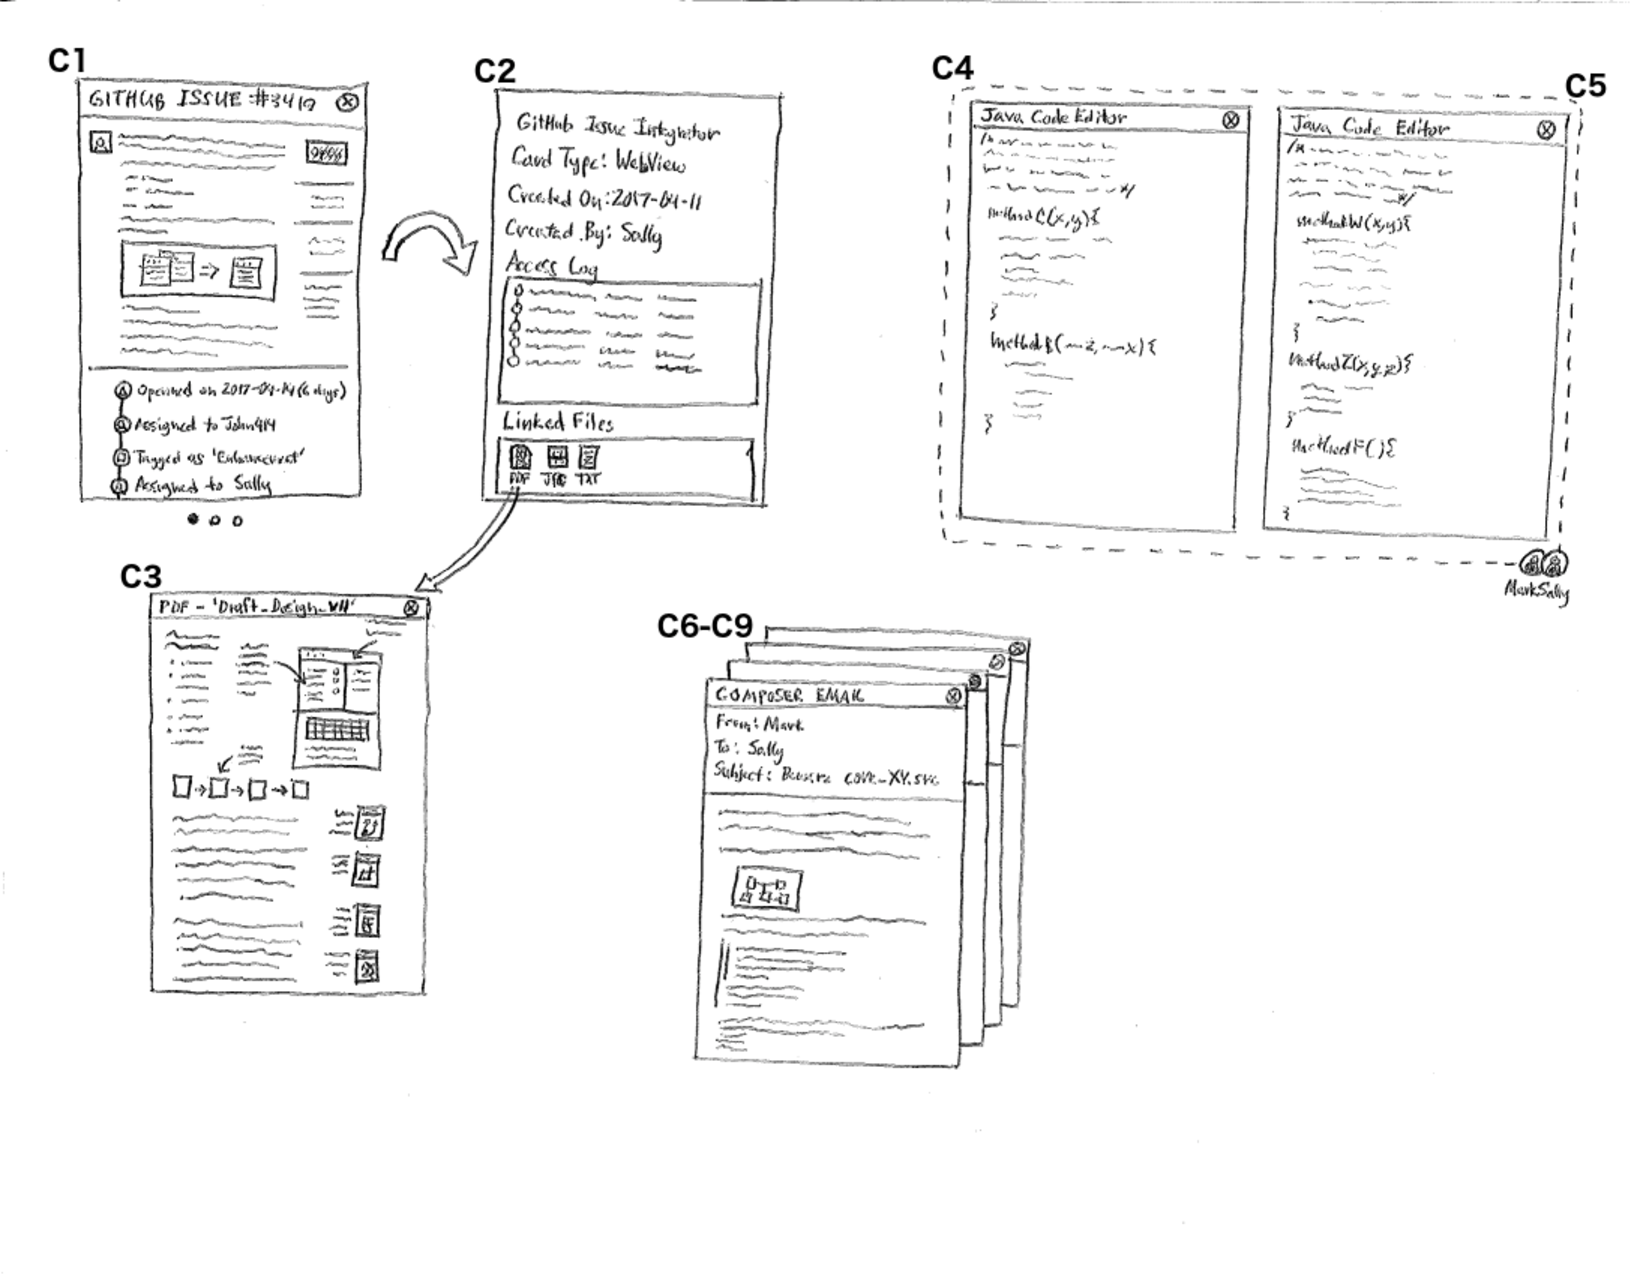
\includegraphics[trim={0.6cm 3.2cm 0.5cm 0.6cm},clip,width=\textwidth]{Mockup-9}}
	\vspace*{-1.5\baselineskip}
\end{figure}

To illustrate our proposed IDE, we present Figure~\ref{mockup} as an illustration of cards used by Sally to accomplish her task using our cards-based user interface.
We describe the scenario in which Sally is tasked with updating a feature to use a new API, but reimagined to use an IDE based on the problem-solving perspective.

Sally initially opens a GitHub Integration card (\texttt{C1}) that retrieves information through the GitHub API and formats the results for a condensed presentation of the description, tags, issue status, and activity history.
The related issue on GitHub contains more activity events than can be presented on the card, and therefore an overflow indicator (three dots below the card) appears to give a visual cue that further information can be accessed via a swiping interaction.
Since Sally is interested in filling in her knowledge gaps about the issue, and any prior knowledge available, she elects to flip the card around and examine the metadata related to card \texttt{C1}.
The reverse card face (\texttt{C2}) contains meta-information related to when the card was created within the IDE, card type, creator, access logs for the card, and any linked files.
Selecting the PDF \texttt{``Draft\_Design\_v11''}, Sally is able to launch a new PDF Viewer card (\texttt{C3}) that contains the sketches and notes from the design team.
She could also open a Text Viewer card and an Image Viewer card for the requirements list from the marketing team and timeline from the project manager from within the linked files section of \texttt{C2}.

Once Sally has grasped the available prior knowledge, contextualized it according to her task, and begun to develop strategies for completing the task she can open additional cards for code exploration and development.
Opening a Java Code Editor card (\texttt{C4}) that contains the target area of code that she will be modifying allows her to simultaneously reference documents from her previous information gathering while working on the code implementation.
Since Sally is not certain that her current changes will be the final solution, she can open an additional Java Code Editor card (\texttt{C5}) which contains the same target area of code prior to the introduction of her proposed changes (thus reflecting the checked-in version).
When reaching out to Mark, the senior developer on her team, Sally is able to select only the cards relevant to their conversation (\texttt{C4,C5}) and share them with Mark so that he can view them in his own IDE workspace.
These shared cards allow both Sally and Mark to edit code simultaneously and share thoughts and ideas without barriers that inhibit the exchange of shared knowledge.
If Mark, or any of the other stakeholders on the project, is unavailable for connecting to the shared cards and instead sends emails to Sally with ideas, sketches, and code snippets, Sally can open each of those emails in Composer Email cards (\texttt{C6-C9}) directly within her IDE workspace.
She can copy and paste the code snippets from the emails and into the Java Code Editor cards without having to switch between two separate applications and manage multiple associated windows.

This example illustrates the process of \textit{collecting alternative solutions}, 
\textit{assessing the feasibility of the alternative solutions}, \textit{examining the applicability of the alternative solutions}, and finally \textit{recombining and consolidating the best aspects into a new solution}.
Traditional IDEs are incapable of supporting these types of activities without relying upon plugins or additional external applications; which typically adhere to different user interface designs and increasing interoperability complexity.

\section{Discussion}
Our conclusions are ...

\bibliography{bibliography}
\bibliographystyle{apacite} 
\end{document}
